\providecommand{\vmodelFirstSection}[1]{\section{#1}}
\providecommand{\vmodelSecondSection}[1]{\subsection{#1}}
\providecommand{\vmodelThirdSection}[1]{\subsubsection{#1}}

\vmodelFirstSection{Vorgehensmodell}
\begin{figure}[!ht]
	\centering
	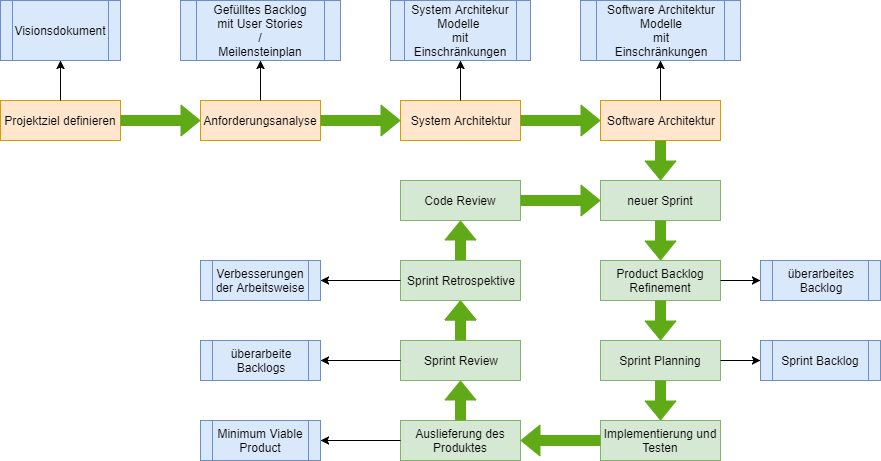
\includegraphics[width=1.0\linewidth]{./ressourcen/vorgehensmodell.png}
	\caption{Vorgehensmodell}
	\label{fig:sec:vorgehensmodell}
\end{figure}
Das Vorgehensmodell der Projektgruppe (siehe \Fig{sec:vorgehensmodell}) besteht aus 2 Abschnitten:
\begin{enumerate}
	\item Wasserfall-ähnliche Definitionsphase
	\item Agile Implementations-und Entwicklungsphase
\end{enumerate}
Die Dokumentation von Entscheidungen und anderen wichtigen Artefakten ist ein fortlaufender Prozess, welcher sich über beide Projektphasen erstreckt.

\vmodelSecondSection{Definitionsphase}
Die am Anfang stattfindende Definitionsphase beinhaltet in chronologischer Reihenfolge folgende Aktivitäten:
\begin{enumerate}
	\item Projektziel definieren
	\item Anforderungsanalyse 
	\item System Architektur definieren
	\item Software Architektur definieren
\end{enumerate}

\vmodelThirdSection{Projektziel definieren}
Während der Aktivität der Projektziel Definition wird ein minimales Projektziel erarbeitet, welches mit allen beteiligten Stakeholdern abgestimmt wurde.
Dieses Projektziel wird in einem \textbf{Visionsdokument} festgehalten, welches ebenfalls eine Einleitung zum Problem enthält und versucht das Projektziel abzugrenzen.

\vmodelThirdSection{Anforderungsanalyse}
Während der Anforderungsanalyse werden die wichtigsten Anforderungen definiert, welche das System umsetzen muss.
Wünsche (Kann-Anforderungen) werden hier ebenfalls notiert, um eine mögliche Erweiterung des Systems zu berücksichtigen.

Bei der Analyse ist jedoch darauf zu achten, dass keine vollständige Erfassung der Anforderungen möglich und erforderlich ist, da während der agilen Entwicklungsphase weitere Anforderungen definiert werden können.
Jedoch ist eine möglichst umfangreiche Analyse zu erreichen, ohne dabei zu viel Zeit verstreichen zu lassen.

Während dieser Analyse wird ein \textbf{Anforderungsdokument} erstellt.
Zudem werden Epics und User Stories definiert, die in einem \textbf{gefüllten Backlog} gepflegt und in das Anforderungsdokument integriert werden.

\vmodelThirdSection{System Architektur definieren}
Hier wird die grundlegende System Architektur definiert.
Diese beschreibt gegebene Schnittstellen und zeigt welche Teil"=Systeme untereinander in welcher Richtung kommunizieren.
Nach dieser Aktivität soll ein Modell erstellt sein, welches die \textbf{Systemarchitektur} darstellt. 

\vmodelThirdSection{Software Architektur definieren}
Während dieser Aktivität werden die Teil"=Systeme genauer definiert und die Schnittstellen ebenfalls.
Nach Beendigung der Aktivität "`Software Architektur definieren"' werden als Artefakte \textbf{Softwarearchitekturen der Teilsysteme} erstellt sein.

\vmodelSecondSection{Entwicklungsphase}
Die Entwicklungsphase wird in mehreren agilen Inkrementen (Sprints) durchgeführt.
Jeder Sprint umfasst die gleichen Aktivitäten in einem typischen Zeitraum von 2-3 Wochen.
\begin{enumerate}
	\item Product Backlog Refinement
	\item Sprint Planning
	\item Implementierung und Testen
	\item Auslieferung des Produktes
	\item Sprint Review
	\item Sprint Retrospektive 
	\item Code Review
\end{enumerate}

\vmodelThirdSection{Product Backlog Refinement}
Während des "`Product Backlog Refinements"' werden besonders die an der Spitze des Backlogs stehenden Epics und User Storys überprüft.
Hier werden insbesondere Schätzungen und Prioritäten überprüft, aber auch Epics werden in kleinere User Storys zerteilt.
Das Refinement des Backlogs hat den Sinn der Reduzierung des Aufwandes während des Sprint Planning, da beim Refinement ebenfalls Abhängigkeiten zwischen verschiedenen User Storys gefunden werden können.

\vmodelThirdSection{Sprint Planning}
Beim Sprint Planning wird entschieden welche User Storys umgesetzt werden.
Zusätzlich wird festgelegt wie die Umsetzung erfolgt und wer sie übernimmt.
Hierfür findet eine Teilung des Sprint Plannings in 2 Phasen statt:
\begin{enumerate}
	\item Festlegung des Was
	\item Festlegung des Wie/Wer
\end{enumerate}

\vmodelThirdSection{Implementierung und Testen}
Während der Implementierung werden die geplanten User Storys und Bugs des Sprints umgesetzt.
Dazu werden in den jeweiligen Teil"=Teams Unteraufgaben erstellt, zu denen ein Zweig im jeweiligen Repositorium angelegt wird.
In diesem werden alle zugehörigen Code"=Änderungen zur Unteraufgabe eingespielt.
Nach Fertigstellung wird ein Pull"=Request in den \textit{develop}"=Branch gestellt, der durch mindestens ein anderes Teammitglied überprüft und genehmigt wird.
Siehe hierzu auch \Fig{sec:vorgehensmodell:branchmodell}.

\begin{figure}[!ht]
	\centering
	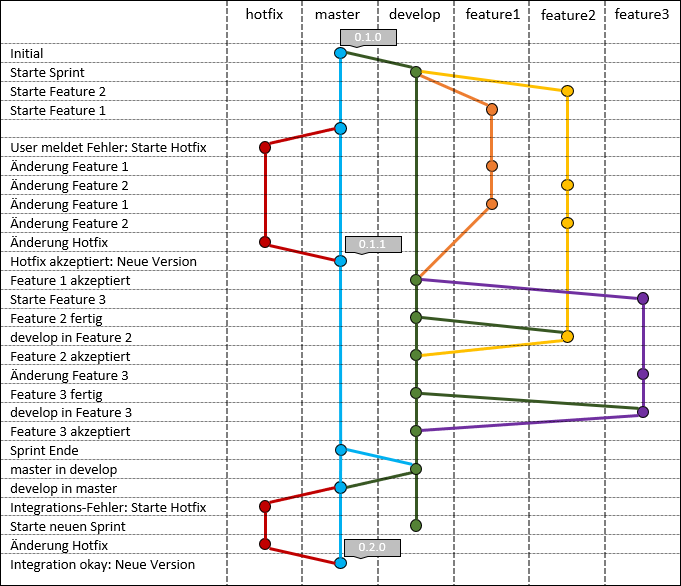
\includegraphics[width=1.0\linewidth]{./ressourcen/Vorgehensmodell_Branchmodell}
	\caption{Branchmodell}
	\label{fig:sec:vorgehensmodell:branchmodell}
\end{figure}

Beim Testen werden einerseits Unit- und Integratiostests im Code geschrieben, die automatisiert ausführbar sind.
Andererseits wird die neue Funktionalität explorativ gegen die Akzeptanzkriterien getestet.
Erst mit bestandenen Tests kann eine User Story abgeschlossen werden.

\vmodelThirdSection{Auslieferung des Produktes}
Nach jedem Sprint Ende wird die erarbeitete Version des Systems "`ausgeliefert"'.
Hierbei wird es sich in der Regel um ein Deployment der überarbeiteten Programme handeln.
Damit im nächsten Sprint mit den Änderungen gearbeitet werden kann.

\vmodelThirdSection{Sprint Review}
Sprint Reviews sind dafür da, um festzustellen, welche User Storys geschafft worden sind und welche noch Arbeit benötigen.
Dieser Schritt hilft, um einen Überblick über den aktuellen Planungs- und Entwicklungsstand zu erhalten.
Darüber hinaus bietet der Review den Steakholdern die Möglichkeit, neue Funktionalitäten vorgestellt zu bekommen und Rückmeldungen sowie Wünsche zu äußern.

\vmodelThirdSection{Sprint Retrospektive}
Während einer Sprint Retrospektive wird die Arbeitsweise während eines Sprints überprüft.
Dafür werden folgende Phasen durchlaufen:
\begin{enumerate}
	\item Informationen sammeln
	\begin{enumerate}
		\item Was lief gut?
		\item Was könnte besser laufen?
	\end{enumerate}
	\item Ursachen herausfinden
	\item Verbesserungsmöglichkeiten bestimmen und anwenden
	\begin{enumerate}
		\item Hier können Aufgaben/Richtlinien entstehen
		\item Änderungen in Projekthandbuch aufnehmen
	\end{enumerate}
\end{enumerate}
Wichtig bei der Retrospektive, aber auch im Allgemeinen ist es ein Arbeitsumfeld zu schaffen, in welchem sich niemand "`schuldig"' fühlt und sich jeder wohl fühlt.

\vmodelThirdSection{Code Review}
Beim Code-Review wird ein Programmabschnitt nach oder während der Entwicklung von einem oder mehreren Gutachtern Korrektur gelesen, um mögliche Fehler, Vereinfachungen oder Testfälle zu finden.
Dabei kann der Gutachter selbst ein Softwareentwickler sein.
Für unerfahrene Entwickler bietet der Code-Review durch einen erfahrenen Programmierer eine gute Möglichkeit, sich schnell und praxisorientiert weiterzubilden.\cite{wiki:codereview}
